\documentclass{standalone}
\usepackage{fontspec}
\setsansfont{DejaVuSans.ttf}[Path=./,Kerning=Off,Ligatures={TeXOff,NoCommon}]
\usepackage{tikz}
\begin{document}
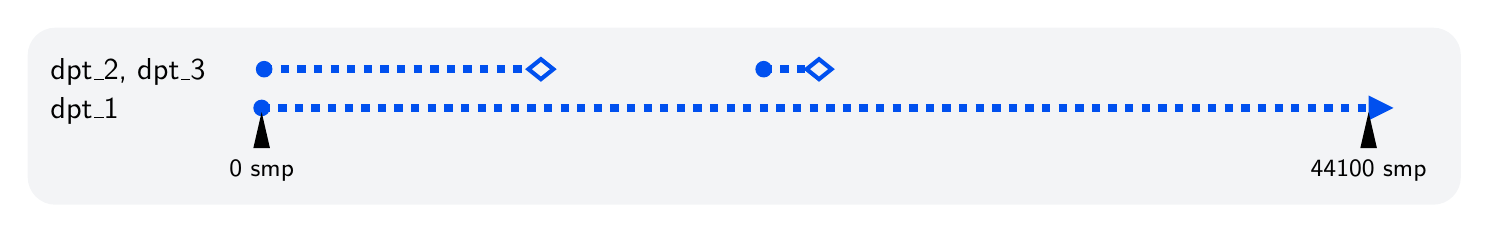
\begin{tikzpicture}[x=1pt,y=1pt,miter limit=4,font=\sffamily]
\definecolor{ts000000}{HTML}{000000}
\definecolor{ts0050EF}{HTML}{0050EF}
\definecolor{tsF3F4F6}{HTML}{F3F4F6}
\begin{scope}[shift={(16,16)}]
\path[rounded corners=10pt,fill=tsF3F4F6] (0,0) rectangle (517.876,63.9766);
\path[draw=ts0050EF,line width=3pt,dash pattern=on 3pt off 3pt] (84.5459,34.9766) -- (484.5459,34.9766);
\path[fill=ts0050EF] (84.5459,34.9766) circle[radius=3];
\path[fill=ts0050EF] (493.5459,34.9766) -- (484.5459,39.4766) -- (484.5459,30.4766) -- cycle;
\path[draw=ts0050EF,line width=3pt,dash pattern=on 3pt off 3pt] (85.4529,48.9766) -- (180.9529,48.9766);
\path[fill=ts0050EF] (85.4529,48.9766) circle[radius=3];
\path[draw=ts0050EF,line width=1.5pt] (180.9529,48.9766) -- (185.4529,52.5766) -- (189.9529,48.9766) -- (185.4529,45.3766) -- cycle;
\path[draw=ts0050EF,line width=3pt,dash pattern=on 3pt off 3pt] (265.9518,48.9766) -- (281.4518,48.9766);
\path[fill=ts0050EF] (265.9518,48.9766) circle[radius=3];
\path[draw=ts0050EF,line width=1.5pt] (281.4518,48.9766) -- (285.9518,52.5766) -- (290.4518,48.9766) -- (285.9518,45.3766) -- cycle;
\path[fill=ts000000] (84.5459,33.4766) -- (81.5459,20.4766) -- (87.5459,20.4766) -- cycle;
\path[fill=ts000000] (484.5459,33.4766) -- (481.5459,20.4766) -- (487.5459,20.4766) -- cycle;
\node[anchor=base west,inner sep=0,font=\sffamily\fontsize{11}{12.8047}\selectfont,text=ts000000] at (8,45.1685) {dpt\_2, dpt\_3};
\node[anchor=base west,inner sep=0,font=\sffamily\fontsize{11}{12.8047}\selectfont,text=ts000000] at (8,31.1685) {dpt\_1};
\node[anchor=base,inner sep=0,font=\sffamily\fontsize{9}{10.4766}\selectfont,text=ts000000] at (84.5459,10.1226) {0 smp};
\node[anchor=base,inner sep=0,font=\sffamily\fontsize{9}{10.4766}\selectfont,text=ts000000] at (484.5459,10.1226) {44100 smp};
\end{scope}
\end{tikzpicture}
\end{document}
